\documentclass{ximera}

%\usepackage{todonotes}

\newcommand{\todo}{}

\usepackage{tkz-euclide}
\tikzset{>=stealth} %% cool arrow head
\tikzset{shorten <>/.style={ shorten >=#1, shorten <=#1 } } %% allows shorter vectors

\usepackage{tkz-tab}  %% sign charts
\usetikzlibrary{decorations.pathreplacing} 

\usetikzlibrary{backgrounds} %% for boxes around graphs
\usetikzlibrary{shapes,positioning}  %% Clouds and stars
\usetikzlibrary{matrix} %% for matrix
\usepgfplotslibrary{polar} %% for polar plots
\usetkzobj{all}
\usepackage[makeroom]{cancel} %% for strike outs
%\usepackage{mathtools} %% for pretty underbrace % Breaks Ximera
\usepackage{multicol}

\usepackage{polynom}



\usepackage[many]{tcolorbox}  %% for titled boxes
\newtcolorbox{xbox}[1]{%
    tikznode boxed title,
    enhanced,
    arc=0mm,
    interior style={white},
    attach boxed title to top center= {yshift=-\tcboxedtitleheight/2},
    fonttitle=\bfseries,
    colbacktitle=white,coltitle=black,
    boxed title style={size=normal,colframe=white,boxrule=0pt},
    title={#1}}


\usepackage{array}
\setlength{\extrarowheight}{+.1cm}   
\newdimen\digitwidth
\settowidth\digitwidth{9}
\def\divrule#1#2{
\noalign{\moveright#1\digitwidth
\vbox{\hrule width#2\digitwidth}}}





\newcommand{\RR}{\mathbb R}
\newcommand{\R}{\mathbb R}
\newcommand{\N}{\mathbb N}
\newcommand{\Z}{\mathbb Z}

%\renewcommand{\d}{\,d\!}
\renewcommand{\d}{\mathop{}\!d}
\newcommand{\dd}[2][]{\frac{\d #1}{\d #2}}
\newcommand{\pp}[2][]{\frac{\partial #1}{\partial #2}}
\renewcommand{\l}{\ell}
\newcommand{\ddx}{\frac{d}{\d x}}
\newcommand{\ddt}{\frac{d}{\d t}}

\newcommand{\zeroOverZero}{\ensuremath{\boldsymbol{\tfrac{0}{0}}}}
\newcommand{\inftyOverInfty}{\ensuremath{\boldsymbol{\tfrac{\infty}{\infty}}}}
\newcommand{\zeroOverInfty}{\ensuremath{\boldsymbol{\tfrac{0}{\infty}}}}
\newcommand{\zeroTimesInfty}{\ensuremath{\small\boldsymbol{0\cdot \infty}}}
\newcommand{\inftyMinusInfty}{\ensuremath{\small\boldsymbol{\infty - \infty}}}
\newcommand{\oneToInfty}{\ensuremath{\boldsymbol{1^\infty}}}
\newcommand{\zeroToZero}{\ensuremath{\boldsymbol{0^0}}}
\newcommand{\inftyToZero}{\ensuremath{\boldsymbol{\infty^0}}}



\newcommand{\numOverZero}{\ensuremath{\boldsymbol{\tfrac{\#}{0}}}}
\newcommand{\dfn}{\textbf}
%\newcommand{\unit}{\,\mathrm}
\newcommand{\unit}{\mathop{}\!\mathrm}
\newcommand{\eval}[1]{\bigg[ #1 \bigg]}
\newcommand{\seq}[1]{\left( #1 \right)}
\renewcommand{\epsilon}{\varepsilon}
\renewcommand{\iff}{\Leftrightarrow}

\DeclareMathOperator{\arccot}{arccot}
\DeclareMathOperator{\arcsec}{arcsec}
\DeclareMathOperator{\arccsc}{arccsc}
\DeclareMathOperator{\si}{Si}
\DeclareMathOperator{\proj}{proj}
\DeclareMathOperator{\scal}{scal}


\newcommand{\tightoverset}[2]{% for arrow vec
  \mathop{#2}\limits^{\vbox to -.5ex{\kern-0.75ex\hbox{$#1$}\vss}}}
\newcommand{\arrowvec}[1]{\tightoverset{\scriptstyle\rightharpoonup}{#1}}
\renewcommand{\vec}{\mathbf}
\newcommand{\veci}{\vec{i}}
\newcommand{\vecj}{\vec{j}}
\newcommand{\veck}{\vec{k}}
\newcommand{\vecl}{\boldsymbol{\l}}

\newcommand{\dotp}{\bullet}
\newcommand{\cross}{\boldsymbol\times}
\newcommand{\grad}{\boldsymbol\nabla}
\newcommand{\divergence}{\grad\dotp}
\newcommand{\curl}{\grad\cross}
%\DeclareMathOperator{\divergence}{divergence}
%\DeclareMathOperator{\curl}[1]{\grad\cross #1}


\colorlet{textColor}{black} 
\colorlet{background}{white}
\colorlet{penColor}{blue!50!black} % Color of a curve in a plot
\colorlet{penColor2}{red!50!black}% Color of a curve in a plot
\colorlet{penColor3}{red!50!blue} % Color of a curve in a plot
\colorlet{penColor4}{green!50!black} % Color of a curve in a plot
\colorlet{penColor5}{orange!80!black} % Color of a curve in a plot
\colorlet{fill1}{penColor!20} % Color of fill in a plot
\colorlet{fill2}{penColor2!20} % Color of fill in a plot
\colorlet{fillp}{fill1} % Color of positive area
\colorlet{filln}{penColor2!20} % Color of negative area
\colorlet{fill3}{penColor3!20} % Fill
\colorlet{fill4}{penColor4!20} % Fill
\colorlet{fill5}{penColor5!20} % Fill
\colorlet{gridColor}{gray!50} % Color of grid in a plot

\newcommand{\surfaceColor}{violet}
\newcommand{\surfaceColorTwo}{redyellow}
\newcommand{\sliceColor}{greenyellow}




\pgfmathdeclarefunction{gauss}{2}{% gives gaussian
  \pgfmathparse{1/(#2*sqrt(2*pi))*exp(-((x-#1)^2)/(2*#2^2))}%
}


%%%%%%%%%%%%%
%% Vectors
%%%%%%%%%%%%%

%% Simple horiz vectors
\renewcommand{\vector}[1]{\left\langle #1\right\rangle}


%% %% Complex Horiz Vectors with angle brackets
%% \makeatletter
%% \renewcommand{\vector}[2][ , ]{\left\langle%
%%   \def\nextitem{\def\nextitem{#1}}%
%%   \@for \el:=#2\do{\nextitem\el}\right\rangle%
%% }
%% \makeatother

%% %% Vertical Vectors
%% \def\vector#1{\begin{bmatrix}\vecListA#1,,\end{bmatrix}}
%% \def\vecListA#1,{\if,#1,\else #1\cr \expandafter \vecListA \fi}

%%%%%%%%%%%%%
%% End of vectors
%%%%%%%%%%%%%

%\newcommand{\fullwidth}{}
%\newcommand{\normalwidth}{}



%% makes a snazzy t-chart for evaluating functions
%\newenvironment{tchart}{\rowcolors{2}{}{background!90!textColor}\array}{\endarray}

%%This is to help with formatting on future title pages.
\newenvironment{sectionOutcomes}{}{} 



%% Flowchart stuff
%\tikzstyle{startstop} = [rectangle, rounded corners, minimum width=3cm, minimum height=1cm,text centered, draw=black]
%\tikzstyle{question} = [rectangle, minimum width=3cm, minimum height=1cm, text centered, draw=black]
%\tikzstyle{decision} = [trapezium, trapezium left angle=70, trapezium right angle=110, minimum width=3cm, minimum height=1cm, text centered, draw=black]
%\tikzstyle{question} = [rectangle, rounded corners, minimum width=3cm, minimum height=1cm,text centered, draw=black]
%\tikzstyle{process} = [rectangle, minimum width=3cm, minimum height=1cm, text centered, draw=black]
%\tikzstyle{decision} = [trapezium, trapezium left angle=70, trapezium right angle=110, minimum width=3cm, minimum height=1cm, text centered, draw=black]


\outcome{Know the graphs and properties of ``famous'' functions.}

\title[Dig-In:]{Working with polynomials}


\begin{document}
\begin{abstract}
  Polynomials are some of our favorite functions. 
\end{abstract}
\maketitle


The functions you are most familiar with are probably polynomial
functions.

\section{What are polynomial functions?}

\begin{definition}
  A \dfn{polynomial function} in the variable $x$ is a function
  which can be written in the form
  \[
  f(x) = a_nx^n + a_{n-1}x^{n-1} + \dots + a_1 x + a_0
  \]
  where the $a_i$'s are all constants (called the \dfn{coefficients})
  and $n$ is a whole number (called the \dfn{degree} when $n\ne
  0$). The domain of a polynomial function is $(-\infty,\infty)$.
\end{definition}

\begin{question}
  Which of the following are polynomial functions?
  \begin{selectAll}
    \choice[correct]{$f(x) = 0$}
    \choice[correct]{$f(x) = -9$}
    \choice[correct]{$f(x) = 3x+1$}
    \choice{$f(x) = x^{1/2}-x +8$}
    \choice{$f(x) = -4x^{-3}+5x^{-1}+7-18x^2$}
    \choice[correct]{$f(x) = (x+1)(x-1)+e^x - e^x $}
    \choice{$f(x) = \frac{x^2 - 3x + 2}{x-2}$}
    \choice[correct]{$f(x) = x^7-32x^6-\pi x^3+45/84$}
  \end{selectAll}
\end{question}

The phrase above ``in the variable $x$'' can actually change.
\[
y^2-4y +1
\]
is a polynomial in $y$, and
\[
\sin^2(x) + \sin(x) -3 
\]
is a polynomial in $\sin(x)$.


\section{Multiplying}

Multiplying polynomials is based on the familiar property of arithmetic, \dfn{distribution}: $\displaystyle a\cdot( b + c ) = ab + ac$.
\begin{example}
	Multiply $2x^3$ by $x^5 - 4x^4 + 7x - 2$.
	\begin{explanation}
		Use distribution.
		\begin{align*}
			2x^3 \left( x^5 - 4x^4 + 7x - 2 \right) &= 2x^3 \cdot x^5 - 2x^3 \cdot 4x^4 + 2x^3 \cdot 7x \\
				& - 2x^3 \cdot 2\\
				&= 2 x^8 - 8x^7 + 14x^4 - 4x^3
		\end{align*}
	\end{explanation}
\end{example}


\begin{example}
	Multiply $3x^2 + 2x - 1$ by $2x^4 + 5x^3+ x + 1$.
	\begin{explanation}
		We'll start by distributing the first polynomial into the second.  Then we'll distribute back, and finish by combining like terms.
		\begin{align*}
			(3x^2+ 2x-1)(2x^4 + 5x^3 + x +1) &= 2x^4(3x^2+ 2x-1) \\
			 &+ 5x^3 (3x^2+ 2x-1) \\
			 &+ x (3x^2+ 2x-1) \\
			 &+ 1(3x^2+ 2x-1)\\
				&= (6x^6 + 4x^5 - 2x^4) \\
				&+ (15x^5 + 10x^4 - 5x^3) \\
				&+ (3x^3+2x^2-x) \\
				&+(3x^2+2x-1)
		\end{align*}
		After combining like-terms, we find \[6x^6 + 19x^5 +8x^4 - 2x^3 + 5x^2+ x - 1.\]
	\end{explanation}
\end{example}
The result is that we have multiplied every term of the first polynomial by every term of the second, then added the results together.  In the case of two
\dfn{binomials} (polynomials with only two terms), this is frequently referred to as \dfn{FOIL}.

There are several product formulas that arise repeatedly when working with binomials.  You will likely have seen most of these before.
\begin{xbox}{Multiplication Formulas}
		\begin{align*}
			(a + b)^2 &= a^2 + 2ab + b^2\\
			(a-b)^2 &= a^2 - 2ab + b^2\\
			(a+b)(a-b) &= a^2 - b^2\\
			(a+b)^3 &= a^3 + 3 a^2 b + 3 ab^2 + b^3\\
			(a-b)^3 &= a^3 - 3 a^2 b + 3 ab^2 - b^3\\
			(a-b)(a^2 + ab + b^2) &= a^3 - b^3\\
			(a+b)(a^2-ab+b^2) &= a^3 + b^3
		\end{align*}
\end{xbox}


\begin{example}
	If $f$ is the polynomial function given by $f(x) = x^3-2x^2 +5$, find $f(x+1)$.  Find $f(2+h)$.
	\begin{explanation}
		$f(x+1)$ means to replace $x$ in the formula for $f(x)$ by $x+1$.
		\begin{align*}
			f(x+1) &= (x+1)^3 - 2(x+1)^2 + 5 \\
				&= (x^3 + 3x^2 + 3x + 1) - 2(x^2 + 2x + 1) + 5\\
				&= x^3 + x^2 -x + 4
		\end{align*}
		In the same way, $f(2+h)$ asks us to replace $x$ by $2+h$.
		\begin{align*}
			f(2+h) &= (2+h)^3 - 2(2+h)^2 + 5\\
				&= (8+12h + 6h^2 + h^3) - 2(4+4h+h^2) + 5\\
				&= h^3 + 4h^2+4h+5
		\end{align*}
	\end{explanation}
\end{example}

\begin{problem}
	If $f(x)=4x^2-3x+1$, find $f(x+h)-f(x)$.
	\begin{multipleChoice}
		\choice{$h$}
		\choice{$4h^2-3h+1$}
		\choice[correct]{$8xh + 4h^2 - 3h$}
		\choice{$4x^2+8xh+4h^2-3x-3h+1$}
	\end{multipleChoice}
\end{problem}

\section{Factoring}
Factoring is a bit like an inverse operation of multiplying polynomials.  We start with the multiplied out polynomial, and ask what the individual factors were.

The easiest factors to deal with are common factors.
\begin{example}
	Factor $8x^5 + 40x^4 + 40x^3$.
	\begin{explanation}
		The coefficients of this polynomial have a greatest common divisor of $8$, and the least degree of the terms is $3$, so
		$8x^3$ is a common factor.  Taking this out leaves:
		$\displaystyle 8x^3( x^2+5x+5)$.
	\end{explanation}
\end{example}


For \dfn{trinomials} (polynomials with three terms) of the form $ax^2 + bx + c$, we try to factor as $(px+r)(qx+s)$.  We'll start with an example with $a=1$.
\begin{example}
	Factor $x^2+2x-24$.
	\begin{explanation}
		Since the leading coefficient is $1$, we want to factor $x^2+2x-24$ as $(x+r)(x+s)$.  If we multiply out $(x+r)(x+s)$ we get
		$x^2 + (r+s)x + rs$.  We need to find two numbers that add to $2$,
		and multiply to $-24$.  Look at the different ways of multiplying two numbers to get $-24$:  $-1 \cdot 24$, $-2 \cdot 12$, $-3 \cdot 8$, $-4 \cdot 6$...
		That last one, $-4$ and $6$ are two numbers that add to $2$ and multiply to give $-24$.
		
		Our factorization is $x^2+2x-24 = (x-4)(x+6)$.
	\end{explanation}
\end{example}

The process is slightly more complicated when $a \neq 1$.
\begin{example}
	Factor $6x^2 + 11 x + 3$.
	\begin{explanation}
		In this case, want to find $(px+r)(qx+s) = pq x^2 + (ps+qr) x+ rs$.  Ignore that middle term for now, and just focus on the leading term and the constant term.
		We need to find numbers that multiply to $6$ for our coefficients, and that multiply to $3$ for the constants in each factor.
		That means we're looking at things like $(6x+1)(x+3)$, $(6x+3)(x+1)$, $(2x+3)(3x+1)$, $(2x+1)(3x+3)$.   Actually, that's it, as $6$ can only
		factor as $1 \cdot 6$ or $2 \cdot 3$, and $3$ only factors as $1 \cdot 3$.
		
		All of these possibilities will give the right $x^2$ term and the right constant term.  The only difference is the $x$-term they give.  Do any of them
		give an $x$-coefficient of $11$?  Yes!
		
		$6x^2+11x+3 = (2x+3)(3x+1)$.
	\end{explanation}
\end{example}

Remember, a \dfn{root} of a polynomial function is an $x$-value where the polynomial is zero. 
There is a close relationship between roots of a polynomial and factors of that polynomial.  Precisely:
\begin{theorem}
If $x=c$ is a root of a polynomial, then $x-c$ is a factor of that polynomial.
\end{theorem}

\begin{example}
	Factor $3x^3-13x^2+2x+8$.
	\begin{explanation}
		Notice that if we substitute $x=1$ into the polynomial, we get zero out.  That means $x-1$ is a factor of $3x^3-12x^2+2x+8$.
		Polynomial long division gives:
		\[\polylongdiv{3x^3-13x^2+2x+8}{x-1}\]
		The quotient was $3x^2-10x-8$, so $3x^3-13x^2+2x+8 = (x-1)(3x^2-10x-8)$.  It remains to factor the quotient.
		
		The leading coefficient $3$ factors as $1 \cdot 3$, and $8$ factors as $1 \cdot 8$ and $2 \cdot 4$.  Examining the possibilities, we find the factorization
		of $3x^2-10x-8$ as $(3x+2)(x-4)$.  The entire polynomial factors as $(x-1)(3x+2)(x-4)$.
	\end{explanation}
\end{example}



\section{Equations}
A \emph{quadratic equation in $x$} is an equation which is equivalent to one with the form
	$ax^2 + bx + c = 0$, where $a$, $b$, and $c$ are constants, with $a \neq 0$.

There are three major techniques you are probably familiar with for solving quadratic equations:
\begin{itemize}
	\item Factoring.
	\item Completing the Square.
	\item Quadratic Formula.
\end{itemize}

Each of these methods are important.  Factoring is vital, because it is a valid approach to solve nearly any type of equation.  Completing
the Square is a technique that becomes useful when we need to rewrite certain types of expressions.  The Quadratic Formula will always
work, but has some limitations.

\begin{example}
	Solve the quadratic equation
	\[ 2x^2 +5x = 27 x - 60. \]
	\begin{explanation}
		We'll start by writing this in it's standard form: $2x^2 - 22x + 60 = 0$.  Notice how there is a common factor of 2? Let's divide by 2.
		
		$x^2 - 11x + 30 = 0$.  Any of the above methods will work here, so let's try factoring.  What numbers add to $-11$ and multiply to $30$?
		$-5$ and $-6$ do. That gives us:
		\begin{align*}
			x^2 - 11x + 30 &= 0\\
			(x-5)(x-6) &= 0
		\end{align*}
		Either $x-5 = 0$ (giving us $x=5$) or $x-6 = 0$ (giving us $x=6$).  The two solutions are $x = 5, 6$.
	\end{explanation}
\end{example}	

\begin{example}
	Solve the quadratic equation
	\[  x^2 = 6x -4.\]
	\begin{explanation}
		Again, we'll write it in standard form: $x^2 - 6x + 4 = 0$.  The quadratic $x^2 -6x+4$ does not factor, so we'll complete the square instead.
		
		Start by moving the constant term to the other side
		\[ x^2 - 6x = -4. \]
		This has $b = -6$.  That means $\displaystyle \dfrac{b}{2} = -3$ and $\displaystyle \left( \dfrac{b}{2}\right)^2 = 9$.  Add $9$ to both sides.
		\[ x^2 - 6x + 9 = -4 + 9 = 5. \]
		The left-hand side is now a perfect square, $\left(x-3\right)^2 = x^2 - 6x + 9$.  We can then solve using square roots.
		\begin{align*}
			x^2 - 6x + 9 &=  5\\
			\left( x-3 \right)^2 &= 5\\
			x-3 = \pm \sqrt{5} \\
			x = 3 \pm \sqrt{5}.
		\end{align*}
	\end{explanation}
\end{example}
If you had used the quadratic formula, $\displaystyle x = \dfrac{-b \pm \sqrt{b^2-4ac}}{2a}$, instead of factoring or completing the square above, you would have found the same solutions.

\begin{problem}
	Solve the quadratic equation $\displaystyle x^2 + 4 = 4\left(x+2\right)$.
	\begin{multipleChoice}
		\choice{$x = \pm 2$}
		\choice[correct]{$x=2\pm 2\sqrt{2}$}
		\choice{$x = -2, -4$}
		\choice{none of the above}
  \end{multipleChoice}
\end{problem}




Building on these methods, we'll consider more general types of equations.
A polynomial equation is an equation which is equivalent to one of the form $a_n x^n + a_{n-1} x^{n-1} + \dots + a_1 x + a_0 = 0$. 
\begin{example}
	Solve the equation $x^4 = 6x^2 - 4$.
	\begin{explanation}
		Start by rewriting as $x^4 - 6x^2 + 4=0$.  This is not a quadratic equation in $x$, but it IS a quadratic in $x^2$.
		We continue by completing the square.
		\begin{align*}
			x^4 - 6x^2 &= 4 \\
			x^4 - 6x^2 + 9 &= 4 + 9\\
			(x^2 - 3)^2 &= 13\\
			x^2 - 3 &= \pm \sqrt{13}\\
			x^2 &= 3 \pm \sqrt{13}
		\end{align*}
		Either $x^2 = 3 + \sqrt{13}$, or $x^2 = 3 - \sqrt{13}$.  Since $3 - \sqrt{13}$ is negative, only $x^2 = 3 + \sqrt{13}$ is possible.
		
		The only real solutions are $x = \pm \sqrt{3 + \sqrt{13}}$.
	\end{explanation}
\end{example}

Factoring is a process that helps us solve more than just quadratic equations, as long as we first get one side of the equation equal to zero.
\begin{example}
	Solve the equation
	\[ 2x^2 \left( x-4 \right) \left( 2x-5\right)^3 = 0. \]
	\begin{explanation}
		The only way for a product of real numbers to be zero, is for one of the factors to have been zero.
		Here, that means either $2x^2 = 0$, or $x-4 = 0$ or $(2x-5)^3 = 0$.
		This gives us three equations, each substantially less complicated than the original one, to solve.  By solving them, we find
		$x = 0, 4, \frac{5}{2}$.
	\end{explanation}
\end{example}

\begin{example}
	Solve  $2x(2x^2 + 1) = x^2(x +13) - 8$.
	\begin{explanation}
		Start by rewriting the equation as $3x^3-13x^2+2x+8 = 0$.  This is not a quadratic-type equation, so we resort to factoring.
		\begin{align*}
			3x^3-13x^2+2x+8 &= 0\\
			(x-1)(3x^2-10x-8) &= 0\\
			(x-1)(3x+2)(x-4) &= 0
		\end{align*}
		Thus, either $x -1 = 0$ (so $x = 1$), or $3x+2=0$ (so $x = -2/3$), or $x-4 = 0$ (so $x=4$).
		
		The solutions are $x = 1, 4, -3/2$.
	\end{explanation}
\end{example}


The next theorem above is a deep fact of mathematics. The great mathematician Gauss proved the theorem in 1799. 
\begin{theorem}[The Fundamental Theorem of Algebra]\index{Fundamental Theorem of Algebra}
  Every polynomial of the form
  \[
  a_n x^n + a_{n-1} x^{n-1} + \dots + a_1 x + a_0
  \]
  where the $a_i$'s are real (or even complex!) numbers and $a_n \ne 0$ has exactly
  $n$ (possibly repeated) complex roots.
\end{theorem}

Recall that the \dfn{multiplicity} of a root indicates how many times that particular root is repeated.
The Fundamental Theorem of Algebra tells us that a polynomial equation of degree $n$, will have exactly $n$ complex solutions, once multiplicity
is taken into account.  As non-real solutions appear in complex-conjugate pairs  (if our equation has real coefficients), we will always have an even number of non-real
solutions.  That means, taking multiplicity into account, a quadratic equation will have either $2$ or $0$ real solutions.  A cubic equation will have either $3$ or $1$ real
solution.


\begin{problem}

	The equation $x^3 = 3x-2$ has $x=1$ as one solution.  Find another solution.
	
	\begin{prompt}
		\[ x= \answer{-2} \]
	\end{prompt}
	\begin{feedback}
  		Notice that there were only two real numbers that solve this equation.  How is that possible, if we said a cubic equation has to have either
		$3$ or $1$ real solutions?
  	\end{feedback}
\end{problem}









\section{What can the graphs look like?}
Polynomial functions with degree $1$ are referred to as linear polynomials.  This is due to the fact
that such a function can be written as $f(x) = mx + b$.  The graph of such a function is a straight line
with slope $m$ and $y$-intercept at $(0,b)$.

Quadratic functions, written as $f(x) = ax^2 + bx + c$ with $a \ne 0$, have parabolas as their graphs.
\begin{example}
	Sketch the graph of the function $f(x) = \frac{1}{2} x^2 + 2x + 1$.
	\begin{explanation}
		To plot the parabola, we first complete the square to write our function in the form $f(x) = a(x-h)^2 +k$.
		\begin{align*}
			f(x) &= \frac{1}{2} x^2 + 2x + 1 \\
				&= \frac{1}{2} \left( x^2+ 4x \right) + 1\\
				&= \frac{1}{2}\left( x^2 + 4x + 4\right) + 1 - \frac{1}{2} \cdot 4\\
				&= \frac{1}{2} \left( x+2 \right)^2 -1
		\end{align*}
		The parabola we are looking for has vertex at $(-2, -1)$, opens upward (since $1/2 > 0$), and is wider than the standard
		$y=x^2$ parabola.
		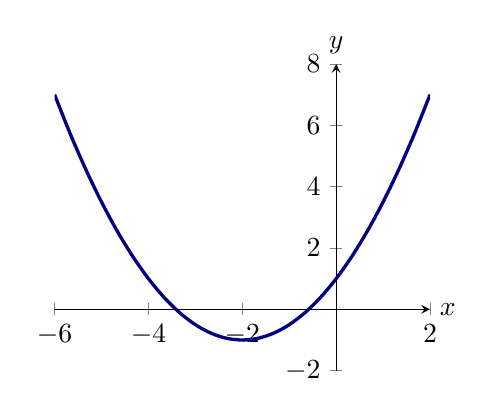
\begin{tikzpicture}
        			\begin{axis}[
          			domain=-6:2,
          			xmin=-6, xmax=2,
          			ymin=-2, ymax=8,
          			width=2.5in,
          			axis lines =middle, xlabel=$x$, ylabel=$y$,
          			every axis y label/.style={at=(current axis.above origin),anchor=south},
          			every axis x label/.style={at=(current axis.right of origin),anchor=west},
          			]
	 	 		\addplot [very thick, penColor, smooth] {0.5*x^2+2*x+1};
        			\end{axis}
      		\end{tikzpicture}
		
		In terms of graph transformations, we can think of this as the graph of $g(x) = x^2$, which has been shifted horizontally $2$ units to the left,
		vertically compressed by a factor of $\frac{1}{2}$, then shifted vertically $1$ unit downward.
	\end{explanation}
\end{example}


\begin{problem}
	Use the graph of $f(x) = 2x^2 - 4x + 3$ to estimate the value of $\lim_{x\to 2} f(x)$.
	\[ \begin{prompt} 
		\lim_{x\to 2} f(x) = \answer{3} 
	\end{prompt}\]
\end{problem} 




The upshot of the Fundamental Theorem of Algebra (in terms of graphing) is that when we plot a
polynomial of degree $n$, its graph will cross the $x$-axis at most
$n$ times.  Each crossing corresponds to a root of that polynomial.

\begin{example}
  Here we see the the graphs of four polynomial functions.
  \begin{image}
    \begin{tabular}{cc}
      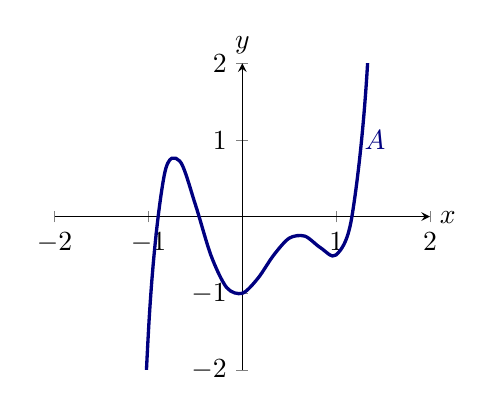
\begin{tikzpicture}
        \begin{axis}[
          domain=-2:2,
          xmin=-2, xmax=2,
          ymin=-2, ymax=2,
          width=2.5in,
          axis lines =middle, xlabel=$x$, ylabel=$y$,
          every axis y label/.style={at=(current axis.above origin),anchor=south},
          every axis x label/.style={at=(current axis.right of origin),anchor=west},
          ]
	  \addplot [very thick, penColor, smooth] {5*x^5-5*x^4-5*x^3+5*x^2+.5*x -1};
          \node at (axis cs:1.2, 1 ) [penColor,anchor=west] {$A$};
        \end{axis}
      \end{tikzpicture}
      &
      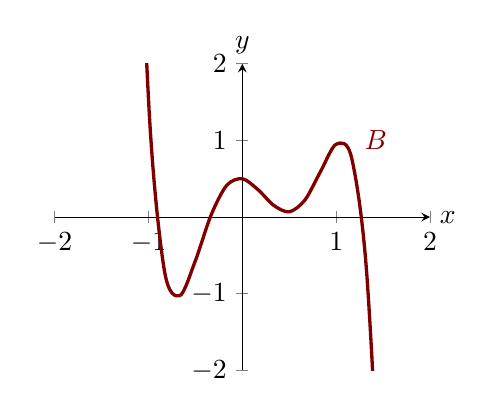
\begin{tikzpicture}
        \begin{axis}[
          domain=-2:2,
          xmin=-2, xmax=2,
          ymin=-2, ymax=2,
          width=2.5in,
          axis lines =middle, xlabel=$x$, ylabel=$y$,
          every axis y label/.style={at=(current axis.above origin),anchor=south},
          every axis x label/.style={at=(current axis.right of origin),anchor=west},
          ]
	  \addplot [very thick, penColor2, smooth] {-5*x^5+5*x^4+5*x^3-4.25*x^2-.3*x +.5};
          \node at (axis cs:1.2, 1 ) [penColor2,anchor=west] {$B$};
        \end{axis}
      \end{tikzpicture}\\
      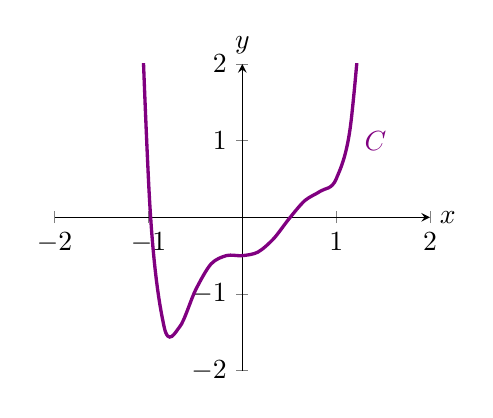
\begin{tikzpicture}
        \begin{axis}[
          domain=-2:2,
          xmin=-2, xmax=2,
          ymin=-2, ymax=2,
          width=2.5in,
          axis lines =middle, xlabel=$x$, ylabel=$y$,
          every axis y label/.style={at=(current axis.above origin),anchor=south},
          every axis x label/.style={at=(current axis.right of origin),anchor=west},
          ]
	  \addplot [very thick, penColor3, smooth] {5*x^6-5*x^5-5*x^4+5*x^3+x^2 -.5};
          \node at (axis cs:1.2, 1 ) [penColor3,anchor=west] {$C$};
        \end{axis}
      \end{tikzpicture}
      &
      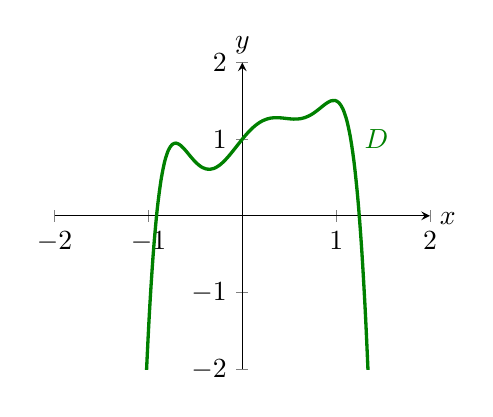
\begin{tikzpicture}
        \begin{axis}[
          domain=-2:2,
          xmin=-2, xmax=2,
          ymin=-2, ymax=2,
          width=2.5in,
          axis lines =middle, xlabel=$x$, ylabel=$y$,
          every axis y label/.style={at=(current axis.above origin),anchor=south},
          every axis x label/.style={at=(current axis.right of origin),anchor=west},
          ]
	  \addplot [very thick, penColor4, smooth,samples=100] {-5*x^6+5*x^5+5*x^4-5*x^3-x^2+1.5*x+1};
          \node at (axis cs:1.2, 1 ) [penColor4,anchor=west] {$D$};
        \end{axis}
      \end{tikzpicture}
    \end{tabular}
  \end{image}
  For each of the curves, determine if the polynomial has
  \textbf{even} or \textbf{odd} degree, and if the leading coefficient
  (the one next to the highest power of $x$) of the polynomial is
  \textbf{positive} or \textbf{negative}.
  \begin{explanation}\hfil
    \begin{itemize}
    \item Curve $A$ is defined by an
      \wordChoice{\choice{even}\choice[correct]{odd}} degree
      polynomial with a \wordChoice{\choice[correct]{positive}\choice{negative}}
      leading term.
    \item Curve $B$ is defined by an
      \wordChoice{\choice{even}\choice[correct]{odd}} degree
      polynomial with a
      \wordChoice{\choice{positive}\choice[correct]{negative}} leading
      term.
    \item Curve $C$ is defined by an
      \wordChoice{\choice[correct]{even}\choice{odd}} degree
      polynomial with a \wordChoice{\choice[correct]{positive}\choice{negative}}
      leading term.
    \item Curve $D$ is defined by an
      \wordChoice{\choice[correct]{even}\choice{odd}} degree
      polynomial with a \wordChoice{\choice{positive}\choice[correct]{negative}}
      leading term.
    \end{itemize}
  \end{explanation}
\end{example}


%% \section{Connections to inverse functions}

%% Polynomials only have inverse functions if they are
%% one-to-one. Pratically this means that polynomials of \textit{even}
%% degree are \textit{never} invertible since they are never
%% one-to-one. Odd degree polynomials may or may not be invertible. This
%% is worth repeating in the language of algebra, and we will write it as
%% a warning.

%% \begin{warning}
%%   Consider $f(x) = x^2$. Suppose we tried to find the inverse of
%%   $x^2$. In this case we plug $f^{-1}(x)$ into $f$ and write
%%   \begin{align*}
%%     f(f^{-1}(x)) &= \left(f^{-1}(x)\right)^2\\
%%     x &= \left(f^{-1}(x)\right)^2
%%   \end{align*}
%% at this point you may be tempted to say ``$f^{-1}(x) = \sqrt{x}$'' but
%% this is not correct. The correct next line is:
%% \[
%% f^{-1}(x) = \pm \sqrt{x},
%% \]
%% but this \textbf{is not a function} from the real numbers to the real
%% numbers.
%% \end{warning}


%% $x^\text{even}$ vs $x^\text{odd}$ and simple nth roots



\end{document}
